\documentclass[sigconf]{acmart}
\usepackage{tikz}
\usepackage{booktabs}
\usetikzlibrary{shapes.geometric, arrows.meta, positioning, fit, calc, backgrounds}

\begin{document}

\title{Cloud-native Disaggregated Storage over RDMA with DISTORT}

\author{Anonymous Author(s)}
\affiliation{%
  \institution{Institution}
  \city{City}
  \country{Country}
}

\begin{abstract}
As cloud-native architectures become the standard for deploying scalable applications, the demand for high-performance, low-latency storage has surged. Disaggregated storage, particularly NVMe-over-Fabrics (NVMe-oF) using Remote Direct Memory Access (RDMA), offers a promising solution by decoupling storage capacity from compute nodes, maintaining near-local access speeds. However, integrating physical RDMA targets with the dynamic, containerized environments of Kubernetes presents significant orchestration challenges. In this paper, we present DISTORT, a Kubernetes-native storage engine designed to bridge this gap. DISTORT leverages a Custom Resource Definition (CRD)-driven state machine to manage the lifecycle of physical NVMe devices, partition them asynchronously, and expose them as NVMe-oF RDMA targets directly to Kubernetes Pods via a Container Storage Interface (CSI) driver. By offloading the control plane to Kubernetes while maintaining a lightweight data path, DISTORT achieves high-performance, dynamic storage provisioning suitable for data-intensive cloud applications.
\end{abstract}

\maketitle

\section{Introduction}
Cloud-native ecosystems, spearheaded by Kubernetes, have revolutionized application deployment through containerization and dynamic orchestration. Traditionally, these environments relied on software-defined storage (SDS) solutions that often introduce overhead via virtualization or user-space file systems. As applications such as machine learning and high-performance databases migrate to the cloud, the overhead of standard SDS becomes a bottleneck.

NVMe-over-Fabrics (NVMe-oF) utilizing RDMA provides microseconds of latency and high throughput, rivaling local NVMe drives. Disaggregating storage using NVMe-oF allows independent scaling of compute and storage resources, improving resource utilization. Yet, orchestrating these high-performance physical targets within Kubernetes without compromising performance or introducing complex middleware is an open challenge.

We introduce DISTORT, a Cloud-native Disaggregated Storage engine over RDMA. DISTORT integrates physical NVMe management directly into the Kubernetes control plane. It introduces an architecture comprising a centralized management controller, a node-level hardware agent, and a standard CSI driver. This design allows Kubernetes to natively declare, partition, and consume bare-metal NVMe storage over RDMA fabrics, utilizing modern user-space polling techniques via SPDK for uncompromised performance.

\section{Related Work}
Recent advancements in distributed storage have focused heavily on integrating high-performance interconnects with cloud-orchestrator frameworks. Systems like SPDK (Storage Performance Development Kit) provide user-space NVMe drivers to bypass kernel overhead, while commercial and open-source CSI drivers (e.g., OpenEBS, Rook/Ceph) offer varying degrees of RDMA support. However, these systems often impose heavy control-plane dependencies or require dedicated storage nodes running complex SDS stacks. DISTORT distinguishes itself by integrating high-performance user-space polling architectures (via SPDK) natively into Kubernetes Custom Resources. It evolved from an initial kernel-based configfs approach to a fully containerized SPDK engine, maintaining a zero-overhead data path without requiring heavyweight SDS middleware.

\section{Design}
DISTORT's architecture is bifurcated into two logical layers: the \textit{NVMe Management Layer} (the "Hardware Control Plane") and the \textit{CSI Layer} (the "Kubernetes Bridge"). This separation of concerns allows the system to decouple physical hardware management from the Kubernetes volume lifecycle using a state-machine-via-CRD approach.

\subsection{Custom Resource Definitions (CRDs)}
At the core of DISTORT's declarative model are four Custom Resource Definitions that mirror the physical and logical state of the storage fabric:
\begin{enumerate}
    \item \textbf{NVMeDevice:} Represents a discovered physical NVMe storage controller on a worker node, including attributes like serial number, NUMA alignment, and block capacity.
    \item \textbf{NVMeDeviceClaim:} Allows administrators or automated provisioners to reserve specific \texttt{NVMeDevice} instances for dedicated workloads.
    \item \textbf{NVMePartition:} Represents a logical slice of an \texttt{NVMeDevice}. It dictates the required capacity and, once scheduled, tracks the NVMe-oF network endpoint details (NQN, Portal IP, Port) required for client connections.
    \item \textbf{RDMAStorageNode:} Represents a worker node's capability to participate in the storage fabric, providing health status and available network interfaces for RDMA traffic.
\end{enumerate}

\begin{figure}[h]
\centering
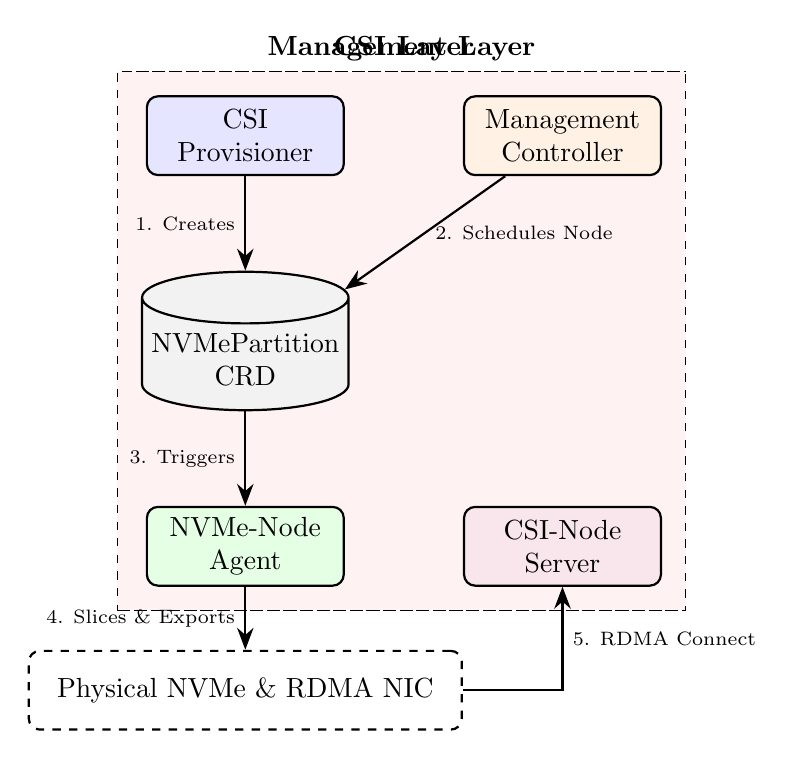
\begin{tikzpicture}[
    node distance=1.2cm and 1.5cm,
    box/.style={rectangle, draw, thick, rounded corners, align=center, minimum width=2.5cm, minimum height=1cm},
    crd/.style={cylinder, draw, thick, aspect=0.25, shape border rotate=90, align=center, minimum width=2cm, minimum height=1cm, fill=gray!10},
    arrow/.style={-{Stealth[scale=1.2]}, thick}
]

% Nodes
\node[box, fill=blue!10] (csiprov) {CSI \\ Provisioner};
\node[crd, below=of csiprov] (crd1) {NVMePartition \\ CRD};
\node[box, fill=green!10, below=of crd1] (agent) {NVMe-Node \\ Agent};
\node[box, fill=orange!10, right=of csiprov] (mgmt) {Management \\ Controller};
\node[box, fill=purple!10, right=of agent] (csinode) {CSI-Node \\ Server};

% Hardware representations
\node[box, dashed, below=0.8cm of agent, minimum width=5.5cm] (hw) {Physical NVMe \& RDMA NIC};

% Background boxes for logical layers
\begin{scope}[on background layer]
    \node[draw, dashed, inner sep=0.3cm, fill=yellow!5, fit=(csiprov) (csinode), label=above:\textbf{CSI Layer}] (csilayer) {};
    \node[draw, dashed, inner sep=0.3cm, fill=red!5, fit=(mgmt) (agent) (crd1), label=above:\textbf{Management Layer}] (mgmtlayer) {};
\end{scope}

% Arrows
\draw[arrow] (csiprov) -- node[left, font=\scriptsize] {1. Creates} (crd1);
\draw[arrow] (mgmt) -- node[right, font=\scriptsize] {2. Schedules Node} (crd1);
\draw[arrow] (crd1) -- node[left, font=\scriptsize] {3. Triggers} (agent);
\draw[arrow] (agent) -- node[left, font=\scriptsize] {4. Slices \& Exports} (hw);
\draw[arrow] (hw.east) -| node[right, near end, font=\scriptsize] {5. RDMA Connect} (csinode.south);

\end{tikzpicture}
\caption{DISTORT Architectural Layers and Interaction}
\label{fig:architecture}
\end{figure}

\subsection{NVMe Management Layer}
This layer is responsible for physical device discovery, disk partitioning, and kernel-level NVMe-oF target exports. It comprises two main components:
\begin{itemize}
    \item \textbf{NVMe-Management-Controller:} Deployed as a centralized replica, it handles administration and placement logic. It reconciles \texttt{NVMeDeviceClaim} objects, allowing cluster administrators to claim specific disks by serial number. Furthermore, when an \texttt{NVMePartition} is requested without a pre-assigned node, this controller selects the optimal \texttt{RDMAStorageNode} based on available free capacity.
    \item \textbf{NVMe-Node-Agent:} Deployed as a DaemonSet across storage-providing nodes. It performs continuous discovery by scanning the PCIe bus for NVMe controllers and reporting active RDMA-capable NICs. Its execution loop watches for \texttt{NVMePartition} CRDs assigned to its resident node, launching \texttt{parted} to slice the physical media and configuring the kernel to expose the partition as an NVMe-oF target.
\end{itemize}

\subsection{CSI Layer (Kubernetes Bridge)}
This layer translates standard PersistentVolumeClaims (PVCs) into concrete storage allocations and subsequently mounts the volumes to application Pods.
\begin{itemize}
    \item \textbf{CSI-Provisioner:} A controller that watches for new PVCs. Instead of communicating with a traditional centralized storage array's backend API, it creates an \texttt{NVMePartition} CRD specifying the required capacity and access mode. It then blocks until the management layer updates the partition's status with an RDMA endpoint (NQN and Portal IP), at which point it binds the resulting PersistentVolume (PV).
    \item \textbf{CSI-Node-Server:} A DaemonSet located on the compute nodes consuming the storage. During the volume staging phase, it executes \texttt{nvme connect} against the NVMe-oF cluster, connecting the Pod to the remote block device (e.g., \texttt{/dev/nvme1n1}). It then bind-mounts this device into the corresponding container's root filesystem.
\end{itemize}

\section{Implementation}
DISTORT is entirely implemented in Go (version 1.23+), leveraging the \texttt{controller-runtime} and Kubebuilder frameworks to enforce operator paradigms. 

\subsection{Codebase Layout \& Components}
The system is compiled into three distinct binary executables situated under the \texttt{cmd/} directory:
\begin{enumerate}
    \item \texttt{distort-manager}: The control plane application housing the claims and placement schedulers.
    \item \texttt{distort-agent}: The privileged hardware-interaction daemon.
    \item \texttt{distort-csi}: Intended to be deployed per the Container Storage Interface spec, containing the Identity, Controller, and Node server gRPC implementations.
\end{enumerate}

Building the binaries relies on a standard \texttt{Makefile} utilizing \texttt{go build}. Kubebuilder macros extract RBAC definitions and scheme topologies from Go structural comments, ensuring that API generations (`\texttt{make manifests}`) directly reflect the Go codebase.

\subsection{Initial Target Implementation}
As the initial proof-of-concept, the \texttt{distort-agent} was designed to interface directly with Linux kernel abstractions to expose NVMe-oF targets without external middleware. 
\begin{itemize}
    \item \textbf{Discovery Mapping:} Probed \texttt{/sys/class/nvme} continuously to calculate NUMA topology and block capacities, translating this into \texttt{NVMeDevice} Custom Resources.
    \item \textbf{Partition Slicing:} Used a wrapper over the \texttt{parted} utility to inject GUID Partition Tables (GPT) and carve primary partitions dynamically.
    \item \textbf{Target Orchestration:} Configured Subsystems, Namespaces, and RDMA Ports strictly by writing to the Linux Kernel's ConfigFS mount (\texttt{/sys/kernel/config/nvmet}).
\end{itemize}

\subsection{SPDK-Based Target Engine}
To significantly elevate I/O performance and reduce CPU overhead from kernel-space context switching, the \texttt{distort-agent} was subsequently upgraded to integrate the Storage Performance Development Kit (SPDK). In this revised high-performance implementation, DISTORT completely bypasses the Linux kernel block layer:
\begin{itemize}
    \item \textbf{User-Space NVMe Driver:} Physical NVMe drives are unbound from the kernel and bound to the \texttt{vfio-pci} or \texttt{uio\_pci\_generic} drivers, granting SPDK exclusive user-space access.
    \item \textbf{Discovery \& RPC Control:} Hardware discovery and telemetry are orchestrated via SPDK's JSON-RPC interface, querying the \texttt{nvmf\_tgt} process for NVMe controllers and serial numbers.
    \item \textbf{Logical Volumes (Lvol):} Instead of traditional filesystem partitions via \texttt{parted}, DISTORT dynamically carves out SPDK Logical Volumes (\texttt{bdev\_lvol\_create}) entirely in application memory.
    \item \textbf{NVMe-oF Exporter:} The kernel's ConfigFS RDMA target registries are deprecated in favor of lightweight SPDK JSON-RPC commands that dynamically create user-space NVMe-oF Subsystems and RDMA listeners on the fly.
\end{itemize}
Volume teardown employs Kubernetes \textit{Finalizers}, intercepting \texttt{NVMePartition} deletion events to cleanly un-export the Fabric pathway via RPC before destroying the logical volume.

\subsection{Deployment Mechanics}
To package the solution for end users, DISTORT maintains an integrated Helm Chart (\texttt{deploy/charts/distort}). The chart templates encapsulate:
\begin{itemize}
    \item \texttt{crds/}: Pre-generated API models.
    \item \texttt{manager-deployment.yaml}: Deploying the centralized scheduler with leader election.
    \item \texttt{agent-daemonset.yaml}: A privileged DaemonSet mounting the host's \texttt{/sys}, \texttt{/dev}, and \texttt{/sys/kernel/config} spaces.
    \item \texttt{csi-daemonset.yaml}: Encapsulating the \texttt{distort-csi} NodeServer alongside standard Kubernetes SIG-Storage sidecars (e.g., \texttt{csi-node-driver-registrar}).
\end{itemize}

\subsection{Testing and Validation Methodology}
To ensure the robustness of the storage engine across the entire stack—from hardware discovery to CSI volume provisioning—DISTORT employs a comprehensive end-to-end (E2E) testing framework. The environment is simulated using Vagrant and VirtualBox, provisioning a multi-node K3s cluster. Each virtual node is equipped with multiple virtual NVMe drives and configured with SoftRoCE (\texttt{rdma\_rxe}) to emulate RDMA fabrics without requiring specialized hardware.

The validation suite is built upon the Ginkgo BDD (Behavior-Driven Development) testing framework and orchestrates tests across three functional layers:
\begin{enumerate}
    \item \textbf{Hardware Discovery:} Asserts that the \texttt{distort-agent} accurately detects virtual NVMe disks and publishes corresponding \texttt{NVMeDevice} CRDs.
    \item \textbf{Controller Logic:} Validates the \texttt{distort-manager}'s scheduling decisions, ensuring \texttt{NVMePartition} resources are placed on nodes with sufficient capacity.
    \item \textbf{CSI Provisioning \& Persistence:} Tests the full lifecycle: dynamic PVC creation, NVMe-oF target export via kernel ConfigFS, RDMA connection from the client pod, `ext4` filesystem formatting, and data persistence guarantees upon pod restarts.
\end{enumerate}

\section{Evaluation}
To assess DISTORT's performance, we conducted a series of microbenchmarks using \texttt{fio} (Flexible I/O Tester) to measure throughput and latency for both local and remote storage access.

\subsection{Experimental Setup}
Our testbed consists of three identical worker nodes equipped with AMD EPYC 7551P 32-Core processors, 256\,GB of RAM, and high-performance NVMe drives. One node acts as the DISTORT management plane/compute node, while two nodes act as storage providers (e.g. equipped with Samsung SSD 990 PRO 4\,TB and Samsung SSD 970 EVO Plus 250GB NVMe drives). The machines are interconnected via an RDMA-capable network to facilitate NVMe-oF traffic.

\subsection{Storage Performance Results}
We established performance baselines using the local NVMe device and evaluated DISTORT's disaggregated storage capabilities over RDMA against Mayastor. Table~\ref{tab:performance} summarizes the throughput and latency metrics for 4\,KB random operations and 1\,MB sequential transfers.

\begin{table*}[t]
\centering
\caption{Microbenchmark Performance Results (4\,KB Random and 1\,MB Sequential I/O)}
\label{tab:performance}
\begin{tabular}{l||rr|rr||rr}
\toprule
\textbf{Configuration} & \multicolumn{2}{c|}{\textbf{4\,KB Random Read}} & \multicolumn{2}{c||}{\textbf{4\,KB Random Write}} & \textbf{1\,MB Seq. Read} & \textbf{1\,MB Seq. Write} \\
& IOPS & Latency ($\mu$s) & IOPS & Latency ($\mu$s) & Bandwidth (MB/s) & Bandwidth (MB/s) \\
\midrule
\multicolumn{7}{l}{\textit{Local Storage}} \\
Raw Device & 887,212 & 571 & 846,046 & 600 & 3,559 & 3,379 \\
Local XFS & 887,271 & 569 & 842,382 & 599 & 2,481 & 3,377 \\
Containerized XFS & 887,596 & 569 & 845,084 & 597 & 2,469 & 3,378 \\
OpenEBS Hostpath & 882,029 & 572 & 843,413 & 598 & 2,493 & 3,376 \\
OpenEBS LVM & 826,081 & 611 & 750,091 & 673 & 2,430 & 3,377 \\
\midrule
\multicolumn{7}{l}{\textit{Remote Storage (NVMe-oF RDMA)}} \\
DISTORT & 137,391 & 3,675 & 142,743 & 3,556 & 3,547 & 3,344 \\
Mayastor & 268,795 & 1,876 & 272,487 & 1,851 & 3,551 & 3,373 \\
\bottomrule
\end{tabular}
\end{table*}

\subsection{Local Storage Performance}
As shown in Table~\ref{tab:performance}, directly accessing the raw NVMe block device yields approximately 887k IOPS for 4\,KB random reads and 845k IOPS for 4\,KB random writes, setting the upper-bound baseline. Formatting the drive with XFS and running within an unprivileged Ubuntu container demonstrates negligible overhead, perfectly matching the bare-metal filesystem performance. Provisioning the storage via Kubernetes using OpenEBS Hostpath also introduces minimal overhead. However, switching to OpenEBS LVM introduces a slight degradation in random I/O, dropping to 826k read IOPS and 750k write IOPS. Sequential write bandwidth remains unaffected across all local configurations, though sequential reads on XFS observed a drop to $\sim$2.4\,GB/s.

\subsection{Remote Storage Performance (RDMA)}
To evaluate DISTORT's disaggregated storage capabilities, we compared it against Mayastor, a popular SPDK-based storage engine configured without replication over NVMe-oF RDMA. Our kernel-based approach achieves $\sim$137k IOPS for 4\,KB random reads and $\sim$142k IOPS for 4\,KB random writes. Sequential workloads hit the network/device limits for both DISTORT and Mayastor, delivering $\sim$3.5\,GB/s reads and $\sim$3.3\,GB/s writes.

\subsection{Discussion}
The evaluation in Table~\ref{tab:performance} reflects the \textit{initial} kernel-based implementation of DISTORT, which highlights a stark contrast in random I/O performance between Mayastor and DISTORT. Mayastor roughly doubles the initial DISTORT's IOPS due to its use of the Storage Performance Development Kit (SPDK). SPDK relies on a user-space, polling-mode driver architecture, which continuously polls the NVMe queues for completions, thereby eliminating context switches and interrupt handling overhead at the cost of dedicating whole CPU cores to the storage engine (100\% CPU utilization per polled core).

In contrast, the initial DISTORT utilized the Linux kernel's standard NVMe-oF target and networking stack, which relies on hardware interrupts. While this interrupt-driven approach limits maximum theoretical IOPS for small block transfers (e.g., 4\,KB), it provided excellent sequential bandwidth and avoided monopolizing CPU resources. Recognizing the performance delta for random I/O workloads, our upgraded SPDK-based implementation of DISTORT (detailed in Section 4.3) adopts the same user-space polling architecture as Mayastor. Future benchmarking of the SPDK engine is expected to showcase performance parity with Mayastor—achieving maximum theoretical random IOPS while maintaining DISTORT's native, zero-overhead Kubernetes orchestration model.

\section{Conclusion}
This report presented DISTORT, a novel storage engine designed to seamlessly integrate high-performance, disaggregated NVMe-oF/RDMA storage with Kubernetes. By mapping physical hardware operations to declarative Custom Resources, DISTORT provides dynamic volume provisioning without sacrificing the bare-metal performance characteristics of RDMA, paving the way for data-intensive applications in cloud-native environments.

\bibliographystyle{ACM-Reference-Format}
\bibliography{references}

\end{document}
